%!TEX root = ED_Arvore.tex

\section{Árvores}
\begin{frame}[label=notas]
	Listas encadeadas são estruturas lineares: como incluir hierarquias?
	\pause
	\\\vfill
	\begin{columns}
		\column{.65\textwidth}
			Árvores
			\begin{itemize}
				\item Dados são dispostos de forma hierárquica
				\item Elementos (\alert{nós}):
					\begin{itemize}
						\item raiz (pai) - [ancestrais]
						\item galhos (filhos) - [ancestrais/descendentes]
						\item folhas (terminais) - [descendentes]
					\end{itemize}
			\end{itemize}
		\column{.35\textwidth}\centering
			\begin{tikzpicture}[->]
				\unbalancedbinarytree
			\end{tikzpicture}
	\end{columns}
\end{frame}

\begin{frame}[label=notas]
	\framesubtitle{Definição Recursiva}
	
	\begin{itemize}
		\item Uma árvore é uma coleção de nós
		\vfill
		\item A coleção pode estar vazia, ou consistir de um nó raiz R
		\vfill
		\item Existe um arco direcionado de R para a raiz  de cada subárvore: a 
		raiz de cada subárvore é chamada de filho de R, e R é o pai da raiz de 
		cada subárvore.
	\end{itemize}
	\begin{center}
		\begin{tikzpicture}[->, level distance=2cm]
			\LARGE
			\Tree [ .R  [ .$S_E$ ] [ .$S_D$ ] ]
		\end{tikzpicture}
	\end{center}
\end{frame}

\begin{frame}[label=notas]
	\begin{center}
		\begin{tikzpicture}[->, level distance=16mm, sibling distance=22mm]
			{\Large \extree}
			\node[subtree, line width=1pt,fit=(a) (b) (e) (i), label=above:{Árvore de raiz A}] {};
			\node<2>[subtree,red,fit=(b) (f),label=below:{\textcolor{red}{Subárvore de raiz B}}] {};
			\node<2>[subtree, green,fit=(c),label=below:{\textcolor{green}{Subárvore de raiz C}}] {};
			\node<2>[subtree, purple,fit=(e),label=above:{\textcolor{purple}{Subárvore de raiz E}}] {};
			\node<2->[subtree, blue,fit=(d) (g) (h) (i),label=below:{\textcolor{blue}{Subárvore de raiz D}}] {};
			\node<3>[subtree, blue!75,fit=(h) (i),label=right:{\textcolor{blue!75}{Subárvore de raiz H}}] {};
			\node<3>[subtree, blue!50,fit=(i),label=right:{\textcolor{blue!50}{Subárvore de raiz I}}] {};
		\end{tikzpicture}
	\end{center}
\end{frame}

\begin{frame}[label=notas]
	Características das árvores:
	\begin{itemize}[<+->]
		\item Ordem: número máximo de galhos em um elemento
		\item Caminho: sequência única de arcos  que leva a um nó a partir da raiz.
		\item Comprimento do Caminho: número de arcos no caminho
		\item Nível de um nó: o comprimento do caminho da raiz 
até o nó , que é o número de arcos no caminho.
		\item Altura: raiz mais o máximo número de descendentes
			\subitem{caminho entre a raiz e a(s) folha(s) mais distante(s) + 1}
	\end{itemize}
\end{frame}

\begin{frame}[label=notas]
	\Large
	\begin{center}
		\begin{tikzpicture}[->, sibling distance=17mm]
			\extree
			\uncover<2->{
				\node[right of = a] (z) 	{};
				\node[right of = z] (x) 	{};
				\node[right of = x] (y) 	{};
				\node[right of = y] (w) 	{};
				\node[right of = w] (n0)	{Nível 0}
				    child {node (n1) {Nível 1} edge from parent[draw=none]
						child {node (n2) {Nível 2} edge from parent[draw=none]
							child {node (n3) {Nível 3} edge from parent[draw=none]}
						}
					}
				;
			}
		\end{tikzpicture}
	\end{center}
	\uncover<2->{Ordem: 4, Altura: 4}
\end{frame}